
%(BEGIN_QUESTION)
% Copyright 2013, Tony R. Kuphaldt, released under the Creative Commons Attribution License (v 1.0)
% This means you may do almost anything with this work of mine, so long as you give me proper credit

Carbon dioxide gas (CO$_{2}$) is a strong absorber of certain infra-red light frequencies.  Knowing this, I once attempted to build my own CO$_{2}$ gas analyzer using the following apparatus:

$$\includegraphics[width=15.5cm]{i00563x01.eps}$$

Testing this apparatus on three known sources of CO$_{2}$, I measured very unexpected results:

% No blank lines allowed between lines of an \halign structure!
% I use comments (%) instead, so that TeX doesn't choke.

$$\vbox{\offinterlineskip
\halign{\strut
\vrule \quad\hfil # \ \hfil & 
\vrule \quad\hfil # \ \hfil & 
\vrule \quad\hfil # \ \hfil \vrule \cr
\noalign{\hrule}
%
% First row
{\bf Gas source} & {\bf CO$_{2}$ content} & {\bf Photodiode output voltage} \cr
%
\noalign{\hrule}
%
% Another row
Ambient air & Weak & Moderate \cr
%
\noalign{\hrule}
%
% Another row
Exhaled air (breath) & Moderate & Weak \cr
%
\noalign{\hrule}
%
% Another row
Pure CO$_{2}$ & Strong & Strong \cr
%
\noalign{\hrule}
} % End of \halign 
}$$ % End of \vbox

My ambient air source was from a compressed air line in a shop.  My pure CO$_{2}$ source was from a high-pressure ``bottle'' of carbon dioxide gas used for MIG welding.

\vskip 10pt

Identify how the photodiode's output voltage {\it should} have responded if this apparatus were indeed sensing CO$_{2}$ content.  Next, hypothesize what this apparatus {\it was} detecting, if not CO$_{2}$.

\underbar{file i00563}
%(END_QUESTION)





%(BEGIN_ANSWER)

This is what the response should have been, if CO$_{2}$ was indeed what was being sensed:

% No blank lines allowed between lines of an \halign structure!
% I use comments (%) instead, so that TeX doesn't choke.

$$\vbox{\offinterlineskip
\halign{\strut
\vrule \quad\hfil # \ \hfil & 
\vrule \quad\hfil # \ \hfil & 
\vrule \quad\hfil # \ \hfil \vrule \cr
\noalign{\hrule}
%
% First row
{\bf Gas source} & {\bf CO$_{2}$ content} & {\bf Ideal photodiode output voltage} \cr
%
\noalign{\hrule}
%
% Another row
Ambient air & Weak & {\it Strong} \cr
%
\noalign{\hrule}
%
% Another row
Exhaled air (breath) & Moderate & {\it Moderate} \cr
%
\noalign{\hrule}
%
% Another row
Pure CO$_{2}$ & Strong & {\it Weak} \cr
%
\noalign{\hrule}
} % End of \halign 
}$$ % End of \vbox


%(END_ANSWER)





%(BEGIN_NOTES)

My own hypothesis is that this apparatus was detecting {\it water vapor concentration} rather than CO$_{2}$ concentration, since water vapor has a much larger infra-red absorption band than carbon dioxide and the water vapor content of my three sample sources are a better match for the experimental results: 

% No blank lines allowed between lines of an \halign structure!
% I use comments (%) instead, so that TeX doesn't choke.

$$\vbox{\offinterlineskip
\halign{\strut
\vrule \quad\hfil # \ \hfil & 
\vrule \quad\hfil # \ \hfil & 
\vrule \quad\hfil # \ \hfil \vrule \cr
\noalign{\hrule}
%
% First row
{\bf Gas source} & {\bf H$_{2}$O content} & {\bf Photodiode output voltage} \cr
%
\noalign{\hrule}
%
% Another row
Ambient air & Moderate & Moderate \cr
%
\noalign{\hrule}
%
% Another row
Exhaled air (breath) & Strong & Weak \cr
%
\noalign{\hrule}
%
% Another row
Pure CO$_{2}$ & Weak & Strong \cr
%
\noalign{\hrule}
} % End of \halign 
}$$ % End of \vbox


%INDEX% Measurement, analytical: carbon dioxide
%INDEX% Measurement, analytical: water vapor in air
%INDEX% Chemistry, spectroscopy

%(END_NOTES)


